\section{Data Reduction Schemes as Packet Streams}\label{sec:terminologies}

In order to systematically study the resolution-versus-precision tradeoffs among different data
reduction schemes, it is important to perform fair and consistent comparisons.  In this section, we
develop such a consistent methodology by proposing to model different data reduction schemes as
\emph{streams} of uniformly sized data \emph{packets}, where the original data contains all of the
packets, and any reduction step removes a set of packets (comparable amounts of data).

These data streams are transmitted using a client-server model. At any point, the client is assumed
to have received a subset of packets from the server (in some pre-determined sequential order or 
in some order requested by the client), which can be used to reconstruct an
approximation to the original data. Therefore, to compare different streams, we reconstruct the
original data using the \emph{same number} of packets from each stream, and perform desired tasks on
each of the (approximate) reconstructions. A stream is considered better suited for a given task if
it produces results that are closer to the ``ground truth'', i.e., the reference results computed
from the original data. \Cref{fig:pipeline} gives a schematic view of our data streaming model.

Although both the server and the client in our model can be on the same physical machine, only the
server has full knowledge of the data. Thus, when the client receives a packet, it might not know
where that packet should be deposited. A common solution is to have both the client and the server
agree beforehand on a static ordering of packets, independent of the data. We use the term
\emph{data-independent streams} to refer to streams using such solutions. In contrast, for
\emph{data-dependent streams}, an additional mechanism is needed to inform the client about the
subbands and bit planes of incoming packets. In this paper, we consider both types of streams, as
well as specialized \emph{task-dependent} streams optimized for given tasks (see
\Cref{tbl:streams}).

\begin{figure}[!b]
\centering
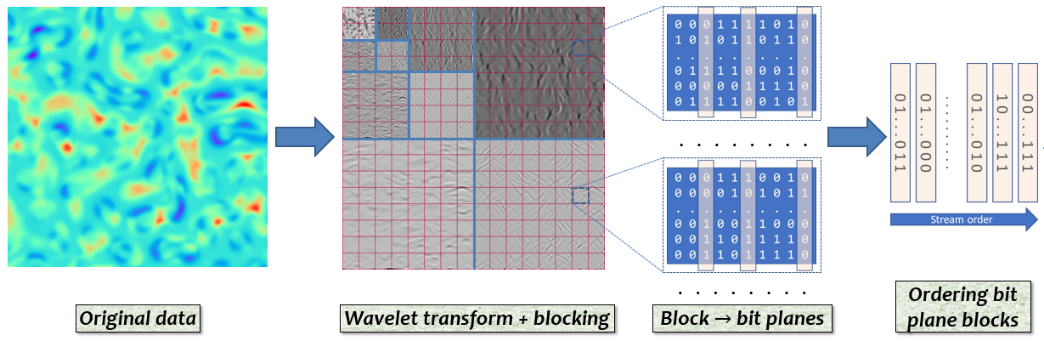
\includegraphics[width=\linewidth]{img/pipeline.png}
\caption{Our data streaming model. The input is a regular grid of floating-point samples;
the output is a stream of \emph{packets}. A packet consists of bits from the same bit plane, from a
block of negabinary wavelet coefficients. Different data reduction schemes generate different
streams.  The wavelet subbands are separated by blue lines in the second image, with the coarsest
subband at the top left corner. 
%Although not shown here, 
Quantization and negabinary convesion
happen immediately after wavelet transform.
%\todo{PL:Please do.  I don’t know what the rightmost two subfigures show.  I also cannot read 1-point font.}
}\label{fig:pipeline}
\end{figure}

\begin{table}[!b]
\setlength\tabcolsep{4.5pt} % default value: 6pt
\centering
\begin{tabular}{l l c c}
\toprule
Symbol & Name & Data Dependent & Task Dependent \\
\midrule
\slvl & \emph{by level} & \xmark & \xmark\\
\sbit & \emph{by bit} & \xmark & \xmark\\
\swav & \emph{by wavelet norm} & \xmark & \xmark\\
\smag & \emph{by magnitude} & \cmark & \xmark\\
\stkop & \emph{task-optimized} & \cmark & \cmark\\
\stksg & \emph{by signature} & \cmark/\xmark & \cmark/\xmark\\
\bottomrule
\end{tabular}
\caption{We define various types of data streams, including data-independent, data-dependent, 
task-independent, and task-dependent streams. \stksg can be data dependent or task
dependent, depending on the stream it derives from.\label{tbl:streams}}
\end{table}

\subsection{Decomposition of Data into Packets} \label{sec:data-streaming-framework}

Although one way to compare different data reduction strategies is to restrict the techniques to the
same data size and compare data quality, it is difficult to enforce consistency. For example, the
amount of change (in data) in one step of multiresolution simplification may be different from
removing one bit in the quantization of every sample. To avoid such mismatch of units of data
increment/decrement, we model each reduction scheme as a stream of equally sized \emph{packets},
which are also the smallest units of data transfer in our framework. A packet consists of a
relatively small number $\left(\approx 2^3\right)$ of bits, and is associated with a resolution
level and a precision level (i.e., bit plane), such that each packet can improve either the
resolution or the precision of data. A resolution-improving packet adds the first bits of
coefficients on a new (and finer) subband locally. In this framework, different data-reduction
schemes become different orderings of packets, called \emph{streams}. Restricting two (or more) data
streams to the same number of packets allows us to perform fair and consistent comparisons.

%\para{Packets for Different Resolution Levels.} 
\para{Resolution Levels.} 
Although there exist several ways to define the notion of resolution/scale/frequency, we choose the
multi-level basis functions of the wavelet transform because they have compact support, and avoid
interpolation problems associated with other representations. Wavelet transform enables spatial
adaptivity (i.e., finer resolution in regions that contain sharp features, at the expense of coarser
resolution elsewhere). In particular, we choose the CDF5/3 multi-linear wavelets~\cite{cdf-wavelets}
for their balance between simplicity and effectiveness at decorrelating the input signal in
practice~\cite{jpeg2000}.

A multidimensional wavelet transform can be performed in multiple passes, which partitions the
original domain into \emph{subbands}, each of which can be thought of as a resolution level
associated with one or more spatial direction. One transform pass (in 3D) creates eight subbands, of
which the first is a low-pass, downsampled version of the original data, and the remaining add fine
details in each subset of the dimensions (see \Cref{fig:pipeline} for a visualization of subbands in
2D). A subsequent transform pass recurses only on the first subband (of the previous level), creating the next (resolution)
level of subbands. We use $l$ $(0 \leq l < L)$ to index the subbands, with $l = 0$ referring to the
coarsest subband and $L$ denoting the number of subbands. In this paper, we use $L=1 + 3*7=22$,
corresponding to three transform passes in 3D.

%\para{Packets for Different Precision Levels.} 
\para{Precision Levels.} 
For creating packets corresponding to different precision levels, we quantize floating-point wavelet
coefficients to $B$-bit signed integers. For most of the experiments in this paper, $B=16$. This
quantization eliminates the floating-point exponent bits, such that every bit (except the sign bit)
can be associated with a bit plane $b$ ($0\leq b < B$). In our convention, the higher indexed bit 
planes are less significant. We convert quantized coefficients to the negabinary representation, where integers are represented in base $-2$, i.e., $\sum_{b=0}^{B}{c_b(-2)^b}$ with $c_b\in \{0,1\}$. 
Negabinary format is preferred over two's complement format, because we start data reconstruction by 
zero-initializing all bits, and negabinary has no single dedicated sign bit and ensures that small coefficients have many leading zero-bits.
%
This transformation increases the number of bit planes by one, i.e., $0\leq b \leq B$ 
(note $\sum_{b=0}^{B}$ in the above expression).
%the summation from $0$ to $B$ in the above expression).

\para{Blocks and Packets.}
Precisely, a \emph{packet} consists of bits from the same bit plane, from a \emph{block} of
negabinary wavelet coefficients. A block is a $[g\times g\times g]$ grid of adjacent coefficients
from the same subband. We let $g$ be a constant ($g=2$ in this paper), so that finer resolution
subbands contain more packets, which presents a tradeoff between packets that provide wider (but
coarser) coverage and packets that provide finer (but more local) details. Every packet (of size one
byte in this paper) comes from a bit plane $b$ and a subband $l$. A packet improves the precision
(or resolution) of a region if it comes from a bit plane (or subband) that has not been streamed
before in the region. $g$ is chosen to be larger than one for performance reason, as in practice,
most systems read bits in batches.

\subsection{Data-dependent and Data-independent Streams} \label{sec:static-dynamic-streams}

We model two common reduction schemes in the literature as \emph{by level} and \emph{by bit plane}
streams. The \emph{by level} stream, \slvl, orders the packets strictly from coarser to finer
subbands. Within the same subband, packets follow the row-major order of blocks and then bit plane
order (from 0 to $B$) within each coefficient. All bits for each coefficient are streamed together.
The other common ordering, \emph{by bit plane}, denoted as \sbit, proceeds strictly from higher
ordered to lower ordered bit planes. Within the same bit plane, packets follow the subband order
(from $0$ to $L-1$), and then row-major order in each subband. The streams \slvl and \sbit are
designed to mimic the way data is accessed in traditional methods that work either in resolution
(\slvl) or in precision (\sbit).

Additionally, we define a third stream that combines these two dimensions and refer to it as
\emph{by wavelet norm}, or \swav. This stream orders packets in descending order of weights
%$\wwav(p)=2^{B-b(p)}\times \norm{\wbas_{l(p)}}^2$,
$\wwav(p)=2^{B-b(p)}\times \| \wbas_{l(p)} \|^2$, 
where $p$ denotes a packet and $\wbas_{l(p)}$
represents wavelet basis on subband $l(p)$. The $||$ notation refers to the $L_2$ norm of the
wavelet basis function. The first term captures the contribution of a bit on bit plane $b(p)$, and
the second term captures the contribution of a wavelet coefficient on subband $l(p)$.
%
% \todo{
% Why the *squared* norm?  This is *not* the contribution of a bit to the error in the function.
% For a wavelet basis function w and associated coefficient $sum c(i) (-2)^i$, bit i (when equal to one) adds a contribution $w (-2)^i$ to the signal.  If you leave this bit out, you'll make an L2 error of $sqrt(||w||^2 (2^i)^2) = ||w|| 2^i$.
% It’s obviously too late to redo the results.  We could perhaps state the correct equation and then fix our results for the revision.  Or we could hope the reviewers find the flaw, and we'll fix it.  Otherwise we have to revise the paper with no reviewer pointing out the flaw.}
%
In the wavelet representation, a function $f$ is written as a linear sum of wavelet basis functions, 
i.e., $f=\sum{c_i\wbas_i}$, where $c_i$ are the coefficients. Since our wavelet transforms
are based on lifting, this norm is usually not one, but increases with level. Basis functions in the
same subband share the same norm, hence $\wwav(p)$ is simply the contribution (in $L_2$ norm) of a
bit on bit plane $b_p$ and subband $l_p$, to the whole function $f$. This ordering based on norms of
wavelet basis functions was proposed previously by Weiss \etal~\cite{weiss}.

Another common way to reduce data in the wavelet domain is to leave out coefficients of smallest
magnitudes. Note that coefficient magnitude is only weakly related to error, as the error also
depends on the wavelet basis function norm~\cite{weiss}. We model this scheme with a stream called
\emph{by magnitude}, or \smag. Here, the weight function is $\wmag(p)=\sum_{c\in
\text{block}(p)}\norm{c}^2$ (the sum is over all coefficients in the block that contains packet
$p$). If two packets have the same weight, they are ordered by subband index, and then by bit plane.

Unlike \slvl, \sbit, and \swav, the \smag stream is data dependent because the coefficient
magnitudes are not known without the data.
%
In principle, data-dependent streams are better than data-independent streams because they can
prioritize important packets based on the actual data. However, data-dependent streams are
ill-suited for practical purposes, because the cost of sending position information likely outweighs
any potential benefit. Nevertheless, we study them for various reasons. First, the \emph{by
magnitude} scheme is well known in literature~\cite{vapor2007}. Second, the ``best'' data-dependent
streams (which do not include position information for packets) can serve as a baseline to evaluate
the performance of their data-independent counterparts. Finally, in addition to being data
dependent, streams can also be task dependent (\Cref{sec:data_dep_streams}), which may provide
insights into how data should be queried to perform certain analysis tasks.

\subsection{Task-optimized Streams} \label{sec:data_dep_streams}

Each analysis task may require a fundamentally different stream for optimal results. Studying such
an ``optimal'' stream is important because it not only serves as a baseline,
but also can provide insights into other, more practical streams for the same task.

Given the original data set $f$ and its reconstructed approximation $\tilde{f}$ using a subset of
packets, let $q$ represent some quantity of interest\footnote{In this paper, we use the terms
``quantity of interest'' and ``task'' interchangeably, with the understanding that, e.g., if the
task is extracting an isosurface, then the quantity of interest is the isosurface.}, e.g.,
histogram, isosurface, etc., computed on $f$ or $\tilde{f}$. For a given task $q$, a well-defined
error metric $\err(q(\tilde{f}),q(f))$ is needed. Given a data set $f$, a task $q$, and an error
metric $\err$, our goal is to generate an \emph{optimal} (and data-dependent) stream, $\sopt$, for
$q$ with respect to $\err$. One possible definition for $\sopt$ is a stream such that the area under
the plotted curve of \err, with respect to the number of bits, is minimized for all packets to be
streamed. However, this definition is limited in practice because a stream should be able to
terminate at any point and still produce as small an error as possible.

Instead, we employ a greedy approach to define the optimal stream. We notice through experiments,
however, that a straightforward greedy algorithm can pick unimportant packets too early. For
example, starting with an all-zero reconstruction $\tilde{f}=0$, and an empty stream, we can
repeatedly append new packets to the stream, which when included in the current $\tilde{f}$, would
minimize $\err$ at every step. At some point, the algorithm might pick a packet that introduces the
lowest error, yet contributes very little to improve the quality of $\tilde{f}$ (because more
important packets would increase the error), leading to a nonoptimal stream. To avoid this problem,
we make a modification to this greedy algorithm, and build the stream backwards. We start with a
``lossless'' $\tilde{f}$ (i.e., $\tilde{f}=f$), and at each step we remove the packet that has the
least impact on the error $\err$ from $\tilde{f}$. This modification largely avoids the previous
problem where less important packets were added to \sopt too early, because by starting with the
full (instead of empty) set of packets, our error measurement captures better the importance of
packets.

Unfortunately, such a greedy algorithm is still expensive in practice, as its complexity is at least
$\mathcal{O}(n^2)$, with $n$ being the total number of packets in the data, due to the 2-level
nested loop. For a $nx\times ny \times nz$ volume and a block size that spans $bx\times by\times bz$
samples, $n$ will be $\frac{nx}{bx}\times \frac{ny}{by}\times \frac{nz}{bz}$. Even a small volume,
e.g., $nx=ny=nz=64$ with $bx=by=bz=2$, hence $n^2=32768^2$, will result in a prohibitively high
run time. Therefore, we adopt a simplified version of this algorithm, where only one pass through
the set of $n$ packets is needed. In iteration $i$ ($0\leq i < n$), we disable (set to zero) a new
packet $p_i$ in $\tilde{f}$, compute and record the incurred error $\err_i$, and then enable $p_i$
again at the end of iteration $i$. After $n$ iterations, each packet has an associated weight
$\err_i$. The stream \sopt is simply the sorted list of packets in decreasing order of the
weights. This simplified algorithm has significantly lower running time, while (by observation)
retaining the same quality for \sopt. \Cref{alg:greedy} outlines the approach described above.

\begin{algorithm}[h]
  \caption{Computing a task-optimized stream}
  \begin{algorithmic}[1]
    \Inputs{
			An original function $f$\\
			An unordered set of $n$ packets $P = \{p_i\}$, produced from $f$\\
			A quantity of interest $q$, and an error function $\err$}
		\Initialize{A set of $n$ weights $\Gamma = \{\gamma_i\}$ }
		\For{each packet $p_i$}
			\State $p_i := 0$
      \State $P \rightarrow$ wavelet coefficients \wcof \\
      		\ \ \ \ \ \ \ \ \ \ \ \ (inverse quantization and inverse negabinary transform)
			\State $\wcof \rightarrow f'$ (inverse wavelet transform)
			\State $\gamma_i := \err(q(f'),q(f))$			
			\State Restore $p_i$
		\EndFor
		\State Sort the $p_i$'s in descending order of $\gamma_i$.
		\Output{The $q$-optimized stream, which is the sorted $P$}
	\end{algorithmic}
	\label{alg:greedy}
\end{algorithm}

\subsection{Stream Signatures} \label{sec:stream-signature}
Unlike data-independent streams, data-dependent streams do not impose a static ordering of packets.
To concisely represent and characterize the dynamic ordering of data-dependent streams, we introduce
the notion of a \emph{stream signature}. Any stream can be represented with respect to the
two-dimensional space of resolution (subbands) and precision (bit
planes), i.e., \mbox{$\Lspace_{L,B}=\{(l,b)\ |\ 0\leq l < L,\ 0\leq b \leq B\}$.}

Given a stream, we define its signature $\sgn$ as an $L \times (1+B)$ matrix, where each $(l,b)$
element is associated with $P_{l,b}$, the set of packets belonging to subband $l$ and bit plane
$b$. In particular, $\sgn_{l,b}$, i.e., the $(l,b)$ element of $\sgn$, is an integer in the range
$[0, (1+B)\times L)$, and indicates, on average, the position at which packets in $P_{l,b}$ appears
in the given stream. For example, the signature $\sgn=\bigl[ \begin{smallmatrix}0 & 1 & 4\\
2 & 3 & 5\end{smallmatrix}\bigr]$ indicates that the stream begins with packets that lie on the
first bit plane of the first subband, as $\sgn_{0,0}=0$. Those are followed by packets on the second
bit plane of the first subband ($\sgn_{0,1}=1$), and then the first bit plane of the second subband
($\sgn_{1,0}=2$), and finally, the third bit plane of the second subband ($\sgn_{1,2}=5$). Thus, a
stream's signature shows how the stream traverses the space $\Lspace_{L,B}$, and highlights the
different resolution-versus-precision tradeoffs among streams, especially among \sopt streams
optimized for different tasks. In~\Cref{fig:example-signatures} we visualize the signatures of
\sbit, \slvl, and \swav, defined in~\Cref{sec:data-streaming-framework}.

To compute a stream signature, we partition the whole domain (not individual subbands) into several
\emph{regions}, compute one signature per region, and average these local signatures. Partitioning
is used since it is only when packets are relatively well localized that their relative ordering in
the $\Lspace_{L,B}$ space becomes meaningful. For example, a packet at one corner of the domain may
be streamed before one at an opposite corner, but this fact contains no useful information. We
define a region to be the spatial volume that is covered by a packet in the coarsest subband.
Algorithm~\ref{alg:signature} lists the steps of our approach.

\begin{algorithm}[h]
  \caption{Computing a stream signature}
  \begin{algorithmic}[1]
    \Inputs{
			A stream $P=\{p_i\}$\\}
		\Initialize{Per-region signature matrix $\sgn_r:= 0$\\
		Global signature matrix $\sgn := 0$}
		\For{each packet $p_i$ in $P$}
			\State Let $r$, $b$, $l$ be the region, bit plane, and subband that $p_i$ belongs
			\State $\sgn_r(l,b) := \sgn_r(l,b)+i$
		\EndFor
		\For{each region $r$}
			\State Sort the elements of $\sgn_r$
			\State Assign each element of $\sgn_r$ its index after sorting
			\State $\sgn := \sgn+\sgn_r$
		\EndFor
		\State Sort the elements of $\sgn$
		\State Assign each element of $\sgn$ its index after sorting
		\Output{The signature matrix $\sgn$}
	\end{algorithmic}
	\label{alg:signature}
\end{algorithm}

Finally, a signature can be used to construct a stream which is denoted generically as $\ssig$. This
construction is done by iterating through each element $\sgn(l,b)$ in ascending order, and adding to
the end of \ssig all the packets in $P_{l,b}$. An \ssig captures the behavior (in the $\Lspace_{L,B}$
space) of the stream it derives from, but is stripped from any spatial adaptivity. Hence, when \ssig
is derived from an \sopt, it can serve as a bridge when comparing the resolution-versus-precision
tradeoffs between data-independent and data-dependent streams.

\begin{figure}[t]
\centering
 \subcaptionbox{\label{fig:by-level-signature}\emph{by level} (\slvl)}{{
\includegraphics[width=0.32\linewidth]{SIG-(STATIC)-(BY-LEVEL)-(rmse)}}}
 \subcaptionbox{\label{fig:rmse:diffisivity}\emph{by bit plane} (\sbit)}{{
\includegraphics[width=0.32\linewidth]{SIG-(STATIC)-(BY-BIT-PLANE)-(rmse)}}}
 \subcaptionbox{\label{fig:rmse:plasma}\emph{by wavelet norm} (\swav)}{ {
\includegraphics[width=0.32\linewidth]{SIG-(STATIC)-(BY-WAVELET-NORM)-(rmse)}}}
\caption{Visualization of signatures for \slvl, \sbit, and \swav in 2D. Each signature is a
$10\times 17$ image, corresponding to $10$ subbands (in 2D) and $17$ bit planes. Each $(l,b)$
``cell'' contains a unique value from $0$ to $169$, indicating its ``priority'' in the stream, and
mapped to a white--blue color scale. \slvl streams bits by resolution (from top to bottom), \sbit
streams by precision (from left to right), while \swav mixes precision and resolution.}
\label{fig:example-signatures}
\end{figure}
